\chapter{Analysis}
\label{chap:analysis}

\section{Introduction}

As the search for Supersymmetry continues to come up empty handed, the masses of potentially new particles are pushed to larger and larger scales. One consequence is that the Standard Model particles radiated in their decay should have correspondingly larger and larger momentum. As the momentum of a particle becomes larger the decay products tend to be emitted at smaller angles, eventually reaching the point where we could reconstruct all the decay objects within a single ``fat jet'' reconstructed using the ``anti-kt'' algorithm with a cone size parameter 0.8. We present an analysis searching for hints of new physics beyond the Standard Model in events with one or two Higgs bosons and a large imbalance in the transverse momentum resulting from supersymmetric particles escaping detection. We require the Higgs boson to decay to b-quarks, exploiting the large (57\%) branching fraction to b-quarks. The branching fraction of Z bosons to b-quarks is substantially smaller at 15\%. This analysis built heavily on previously published work \cite{SUS16033} \cite{SUS15002}. To further suppress misidentification of these jets, we further require the invariant mass of the jet to be consistent with the Higgs boson, to improve mass reconstruction, the soft and wide angle radiation is first removed from the jet before the mass calculation.

\section{Event \& Object Selection}

Although our analysis is sensitive to any process which can produce boosted Higgs or Z bosons, we have adopted a couple of benchmark models, seen in Figure \ref{fig:sms}, to give motivation to the region of phase space we work in. In this scenario, the proton-proton interaction produces a pair of gluinos ($\tilde{g}$) which decay to a neutralino ($\chi_{2}^{0}$) by the emission of Standard Model quarks. A small mass splitting between the gluino and neutralino ($\chi_{2}^{0}$) will result in low $p_{T}$ quarks and a high $p_{T}$ neutralino $\chi_{2}^{0}$. This neutralino $\chi_{2}^{0}$ further decays into another neutralino $\chi_{1}^{0}$ with the emission of a Higgs or Z boson. The neutralino $\chi_{1}^{0}$ escapes detection.

\begin{figure}[htbp]

\begin{subfigure}[b]{0.5\textwidth}
\centering
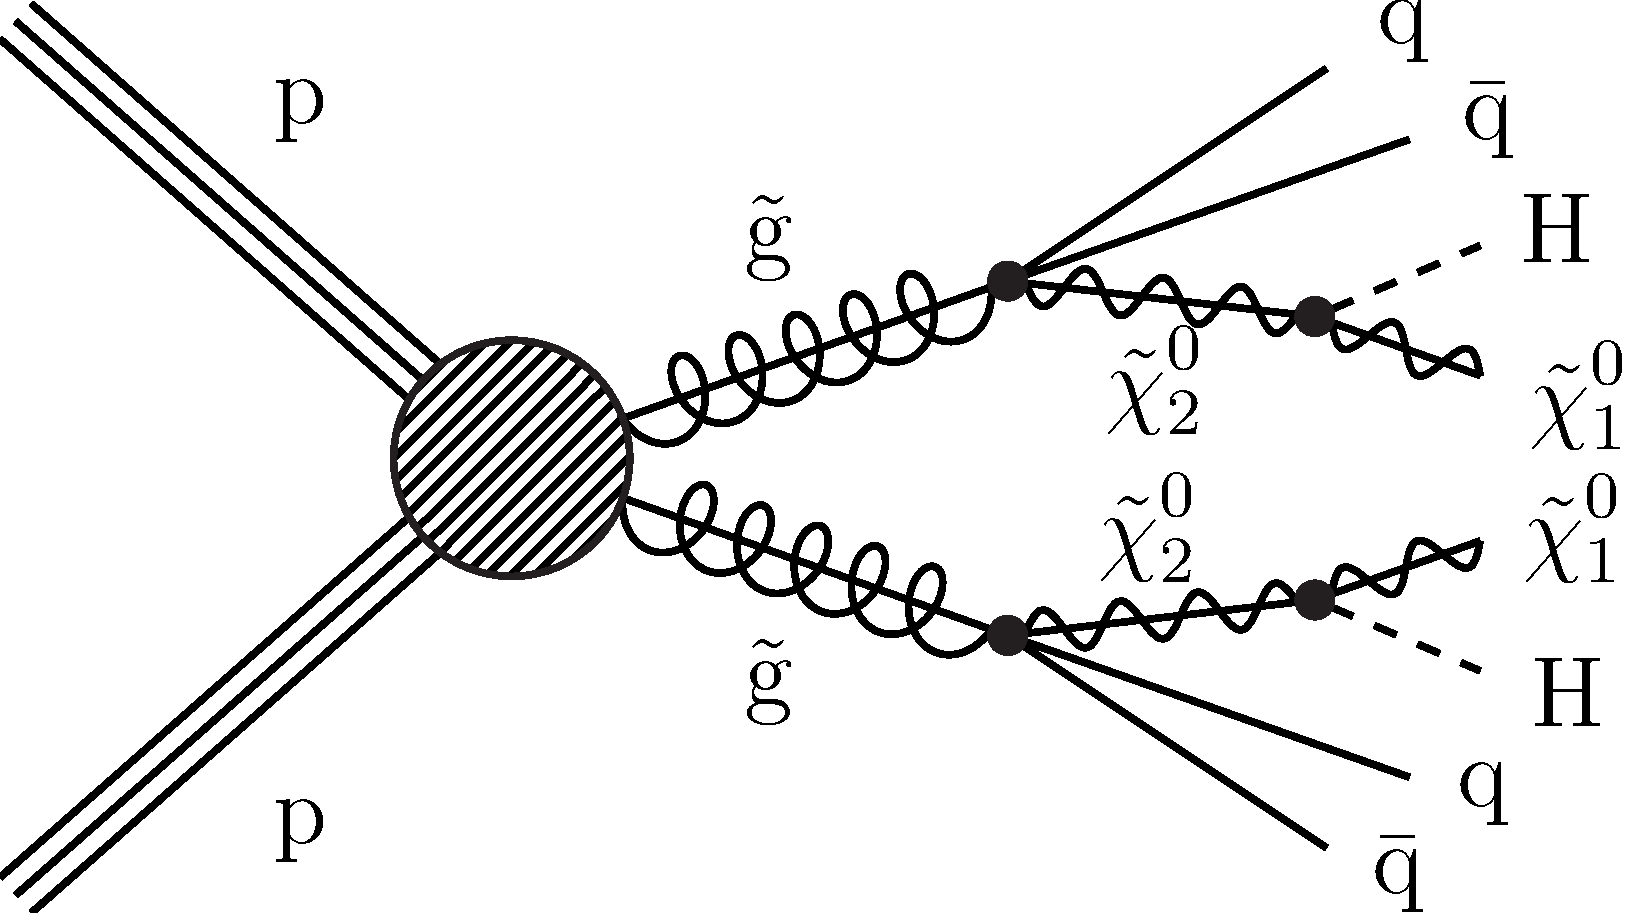
\includegraphics[width=0.5\textwidth]{figs/CMS-SUS-17-006_Figure_001.pdf}
\caption{The T5HH model.}
\end{subfigure}

\begin{subfigure}[b]{0.5\textwidth}
\centering
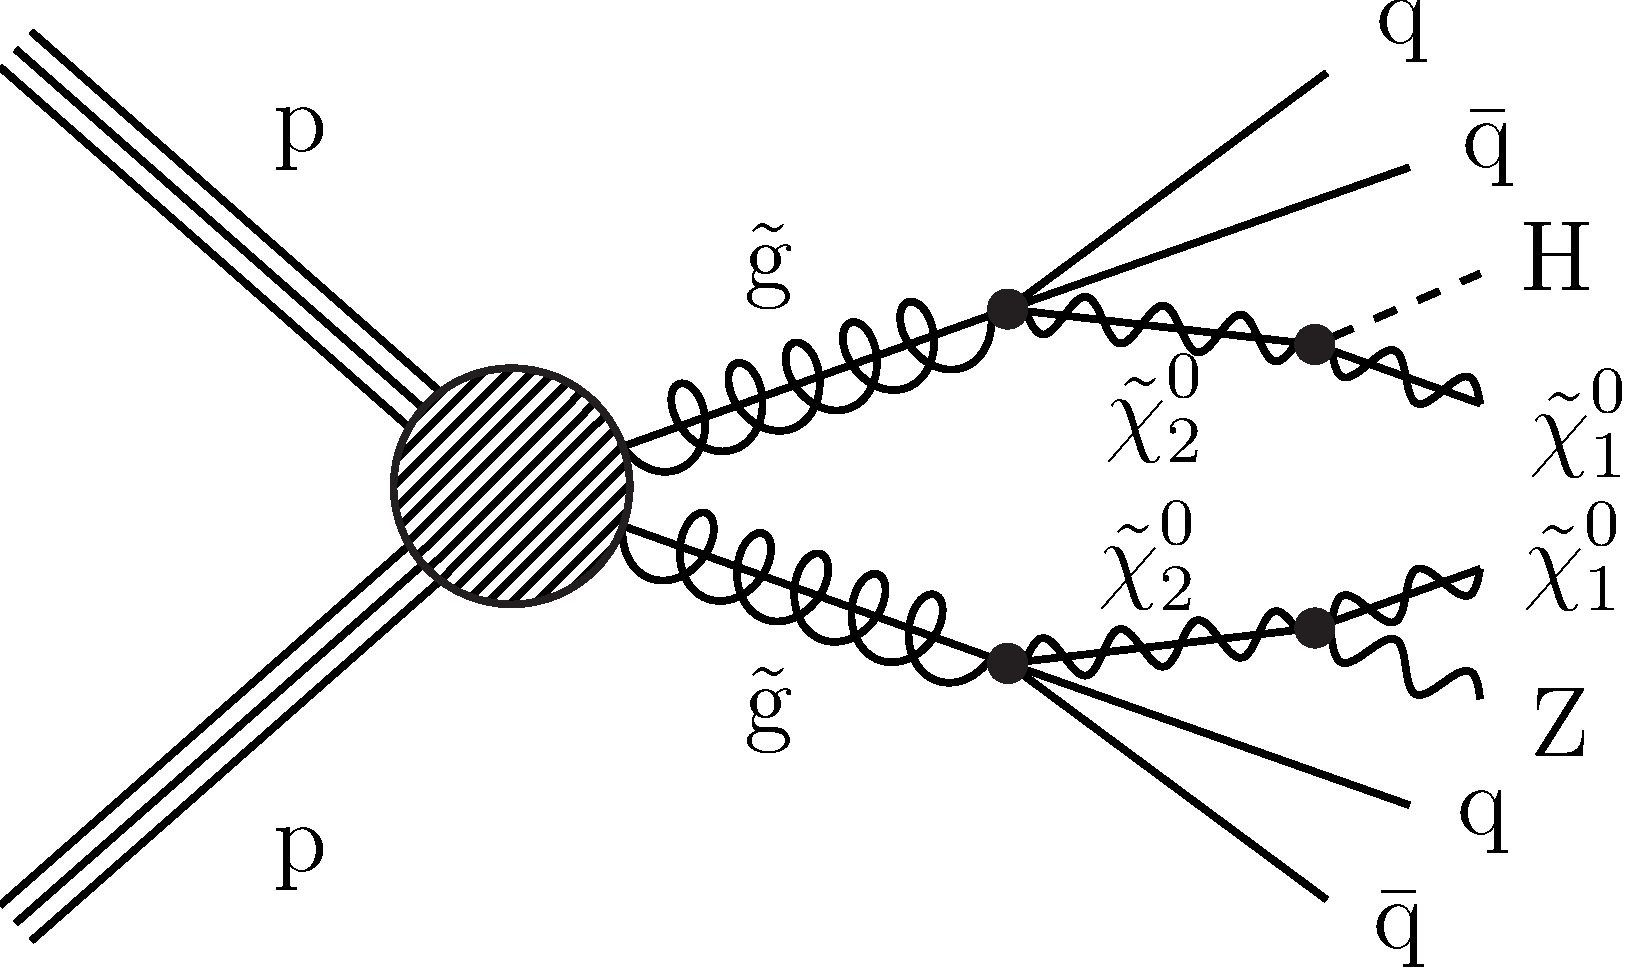
\includegraphics[width=0.5\textwidth]{figs/CMS-SUS-17-006_Figure-aux_001.pdf}
\caption{The T5ZH model.}
\end{subfigure}

\caption{A diagram of the SMS models used for interpretations of this analysis.}
\label{fig:sms}
\end{figure}

The most salient selection criteria is the requirement of at least two high-$p_{T}\,(>300\,\mathrm{GeV}$) AK8 jets.

\section{Background Estimation Procedure}

The background estimation procedure makes use of what is known as an ``ABCD'' prediction where the analysis phase space is divided up into signal and sideband regions using scaling relations to make predictions of the Standard Model background inclusive in all processes. The phase space is divided up according to whether or not the jets are a) in the signal mass region and b) have been tagged as being consistent with a $b\bar{b}$ jet. A diagram of this partitioning is seen in Figure \ref{fig:abcd}. The two signal regions $\mathrm{A}_{1}$ and $\mathrm{A}_{2}$ contain events with one (and only one) or two jets being consistent with Higgs boson decay. Assuming that there is no correlation between the jet mass and the $b\bar{b}$-tagging, the ratio of events $\mathrm{A}_{1, 2} / \mathrm{B}_{1, 2}$ should be the same as $\mathrm{C} / \mathrm{D}$. Rearranging this gives a prediction for the events in the A1 or A2 signal regions, $\left(\mathrm{A}_{1, 2}\right)_{\mathrm{prediction}} = \left(\mathrm{B}_{1, 2} * \mathrm{C} / \mathrm{D}\right)_{\mathrm{observed}}$. The signal regions in data are blinded until the background prediction is made, but we are able to test the closure of our background estimation method in simulation. The closure is seen in Figure \ref{fig:mcclosure}. To account for the non-closure in the signal regions in data a correction factor $\kappa$ is applied to each prediction. The values of $\kappa$ are calculated from a combination of data and simulation. The values can be seen in Table \ref{tab:yieldstable}.

\begin{figure}[htbp]
\centering
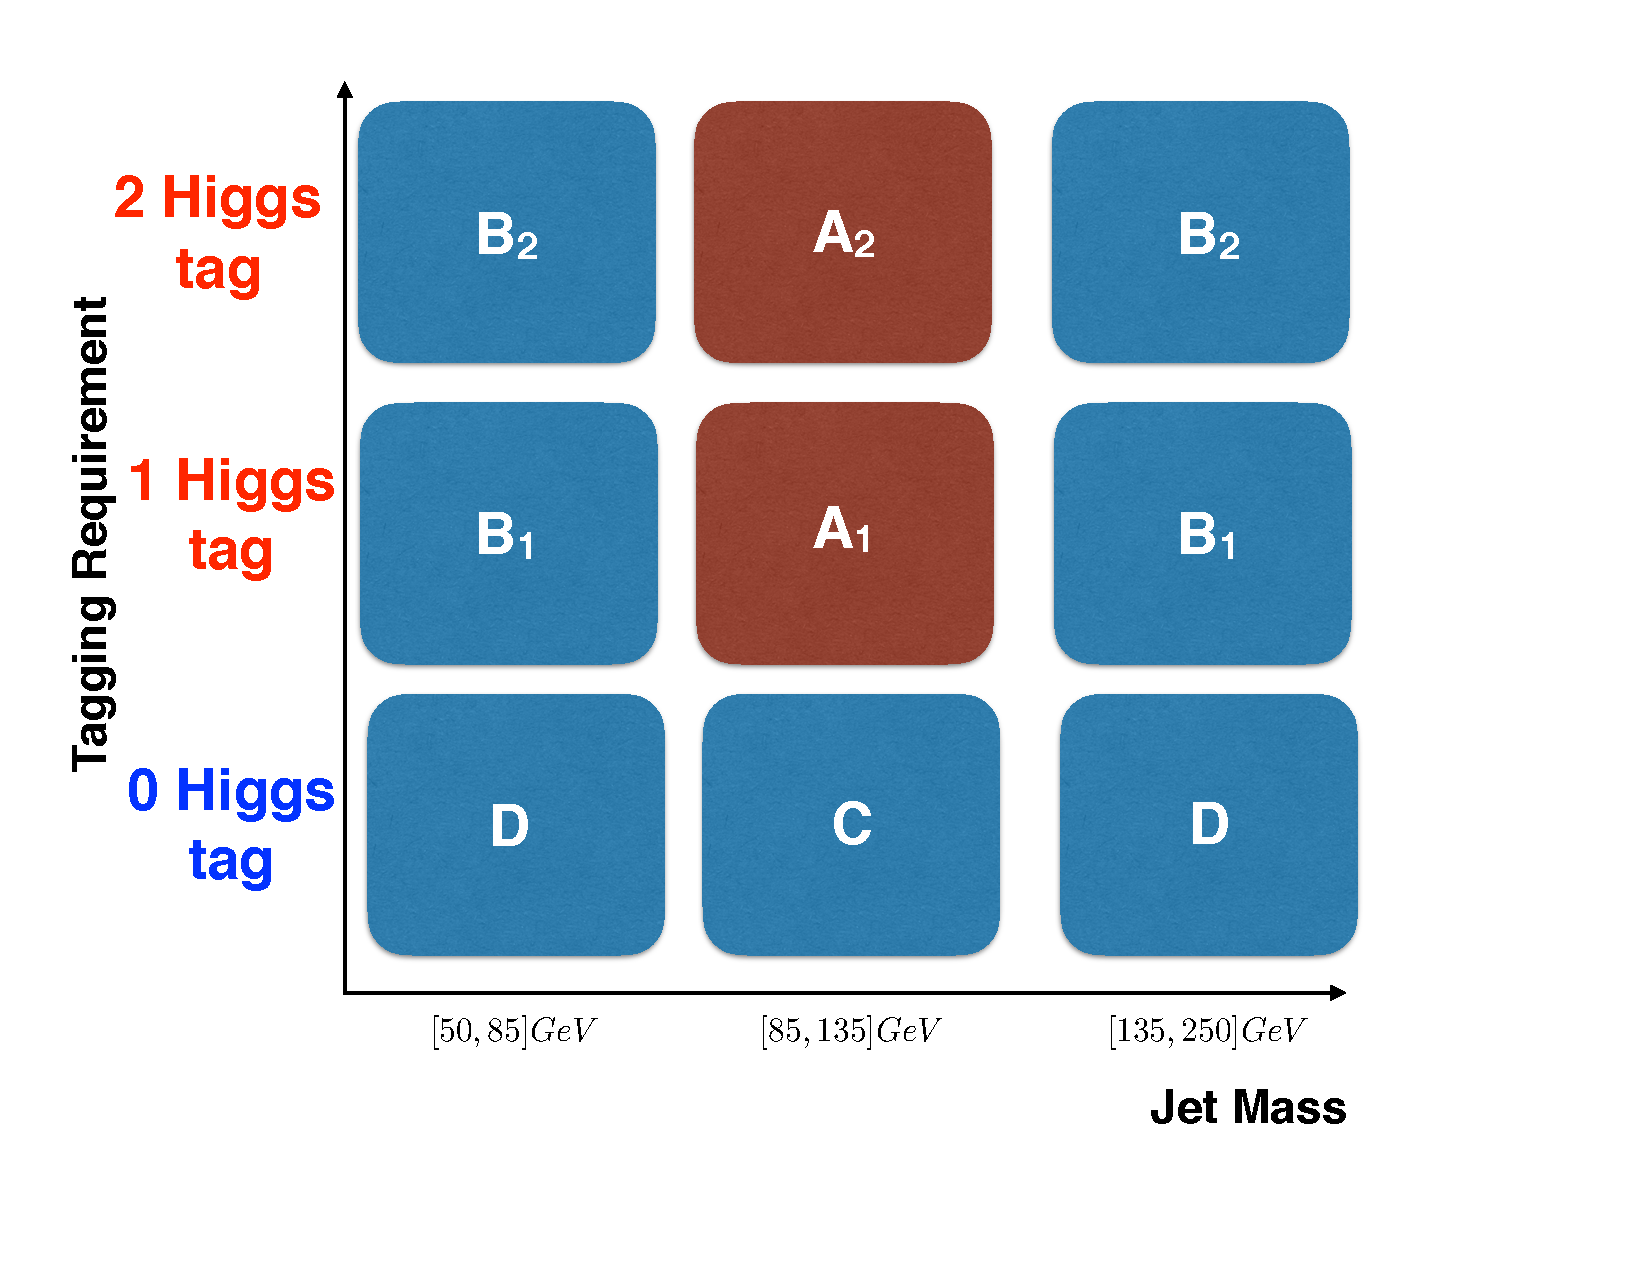
\includegraphics[width=0.75\textwidth]{figs/CMS-SUS-17-006_Figure-aux_002.pdf}
\caption{A diagram of the partitioned phase space.}
\label{fig:abcd}
\end{figure}

\begin{figure}[htbp]

\begin{subfigure}[b]{0.5\textwidth}
\centering
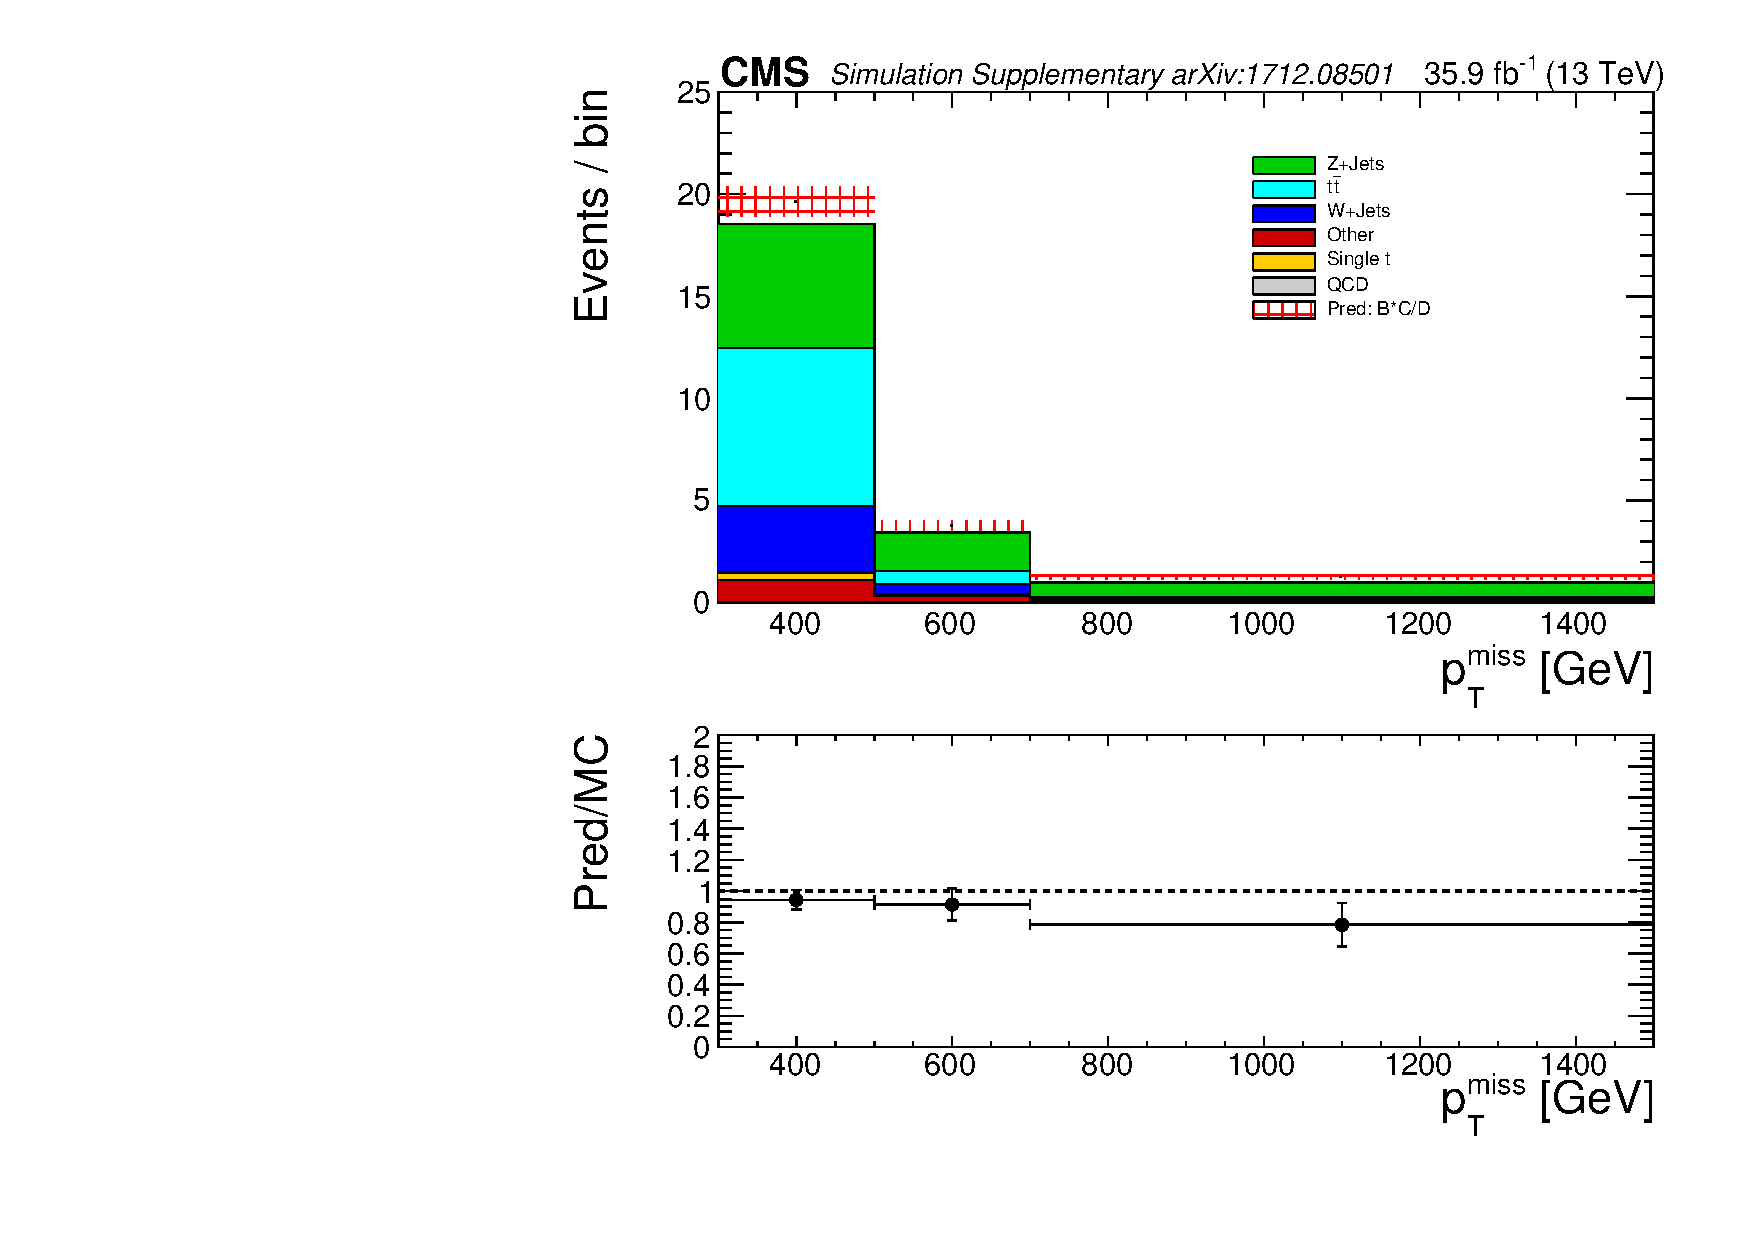
\includegraphics[width=0.75\textwidth]{figs/MCclosure_singleHiggsRegionTotal.pdf}
\caption{The single Higgs tag region (A$_{1}$).}
\end{subfigure}

\begin{subfigure}[b]{0.5\textwidth}
\centering
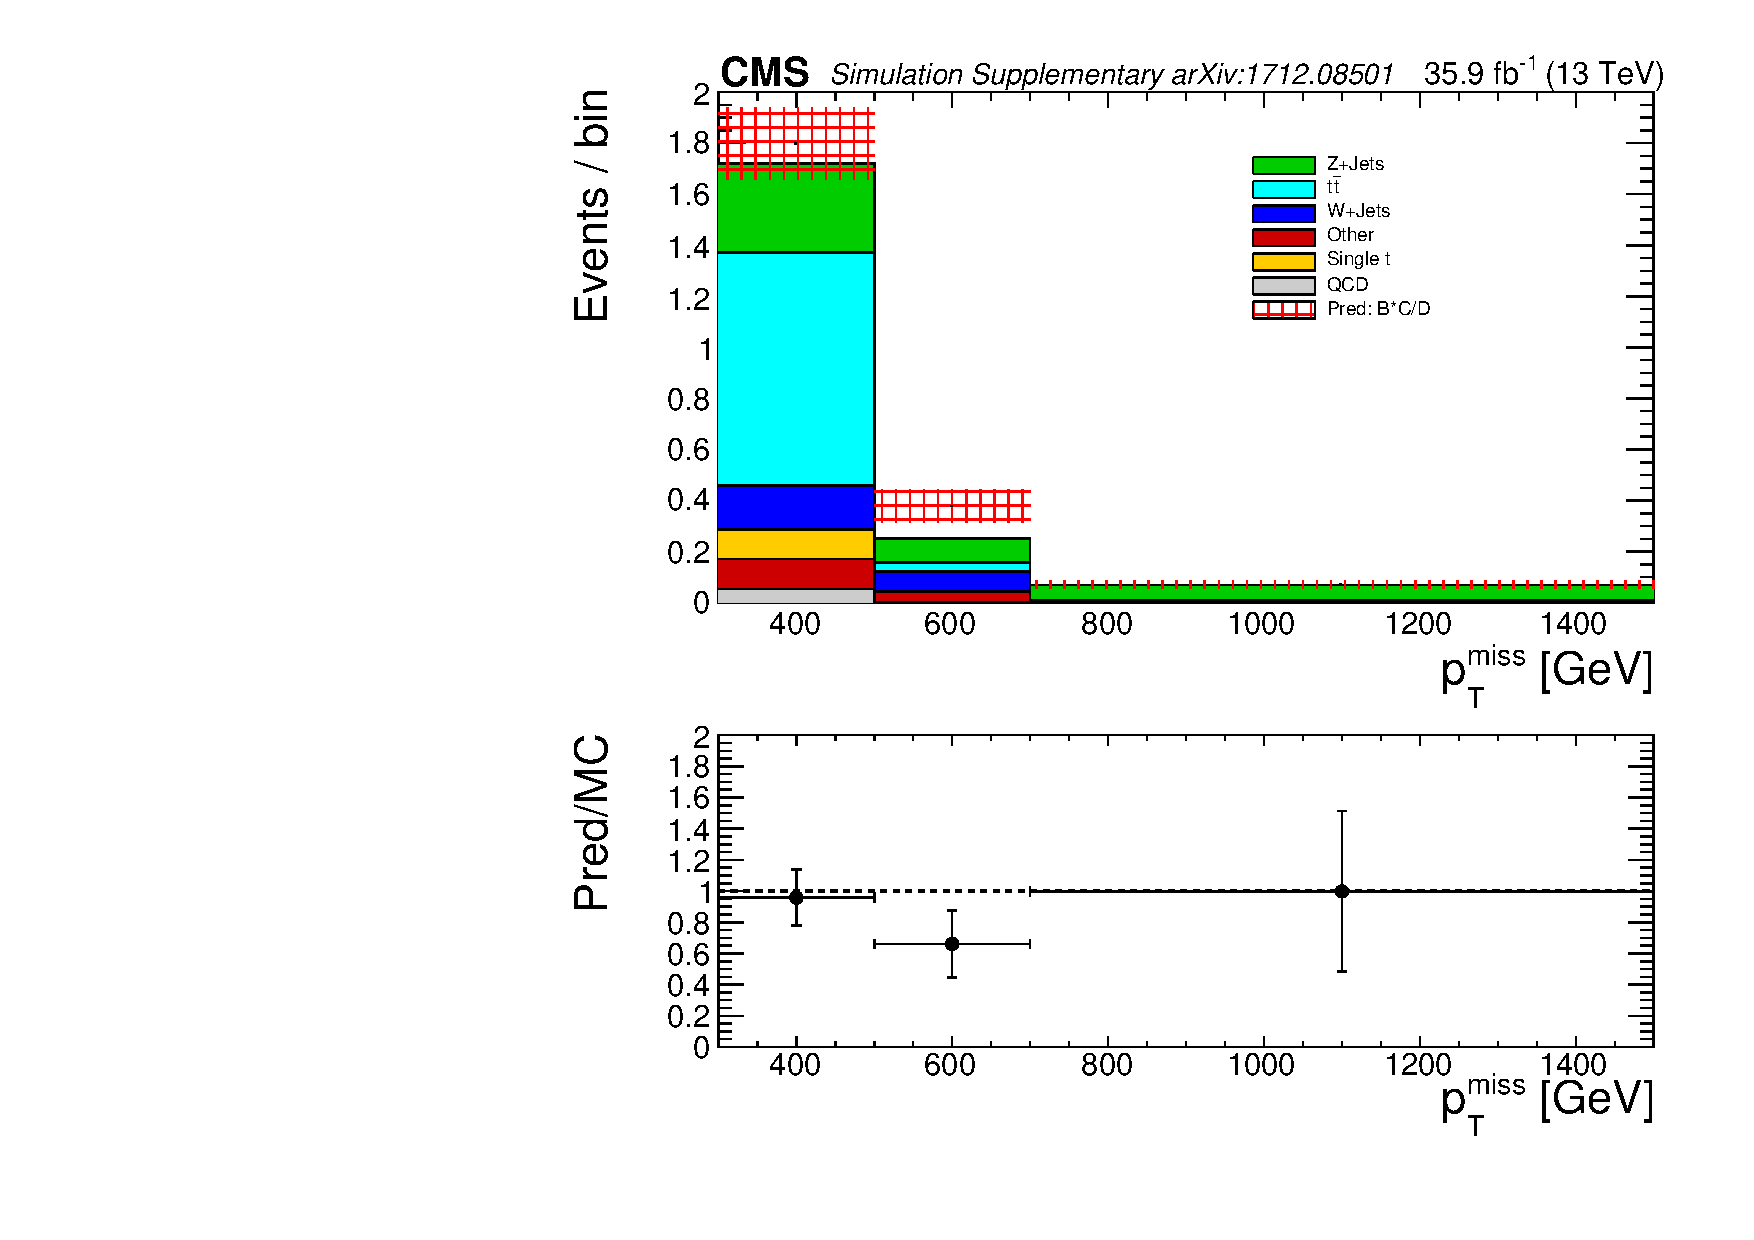
\includegraphics[width=0.75\textwidth]{figs/MCclosure_doubleHiggsRegionTotal.pdf}
\caption{The double Higgs tag region (A$_{2}$).}
\end{subfigure}

\caption{Simulation-based closure in the signal regions.}
\label{fig:mcclosure}
\end{figure}

Yields in these control regions are seen in Figure \ref{tab:yieldstable}, in addition the the yields in the two signal regions.

\begin{table}[htbp]
\centering
\caption{Yields in each of the 6 analysis regions.}
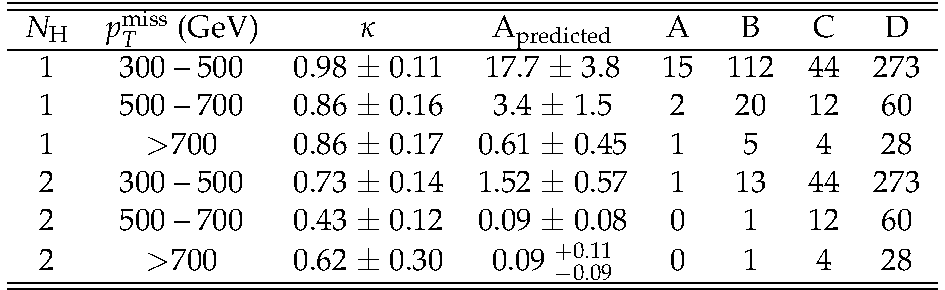
\includegraphics[width=0.75\textwidth]{figs/CMS-SUS-17-006_Table-aux_001.pdf}
\label{tab:yieldstable}
\end{table}

\section{Results}

Observed yields in the two signal regions (A1 \& A2) are seen in Figure \ref{fig:signalyields}. Our signal region yields are consistent with the background expectation.

\begin{figure}[htbp]

\begin{subfigure}[b]{0.5\textwidth}
\centering
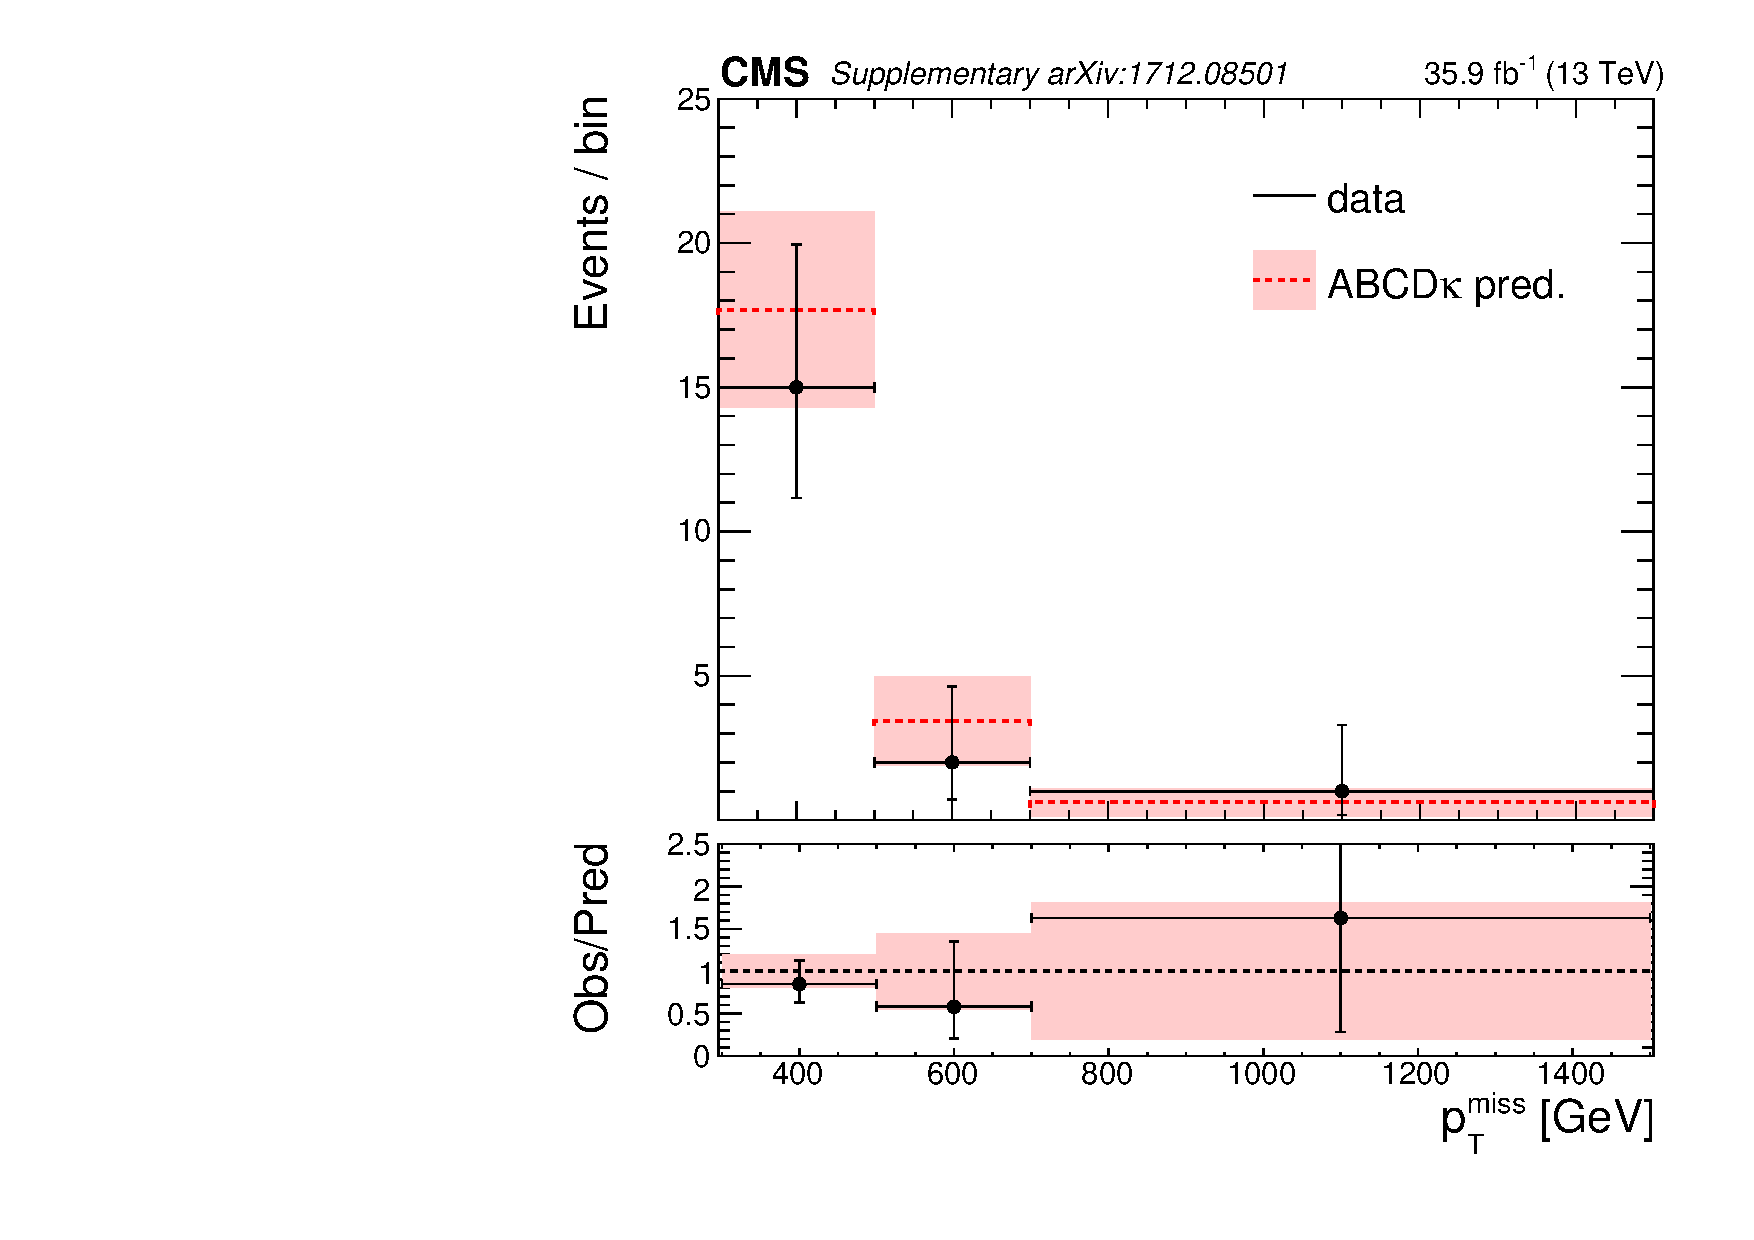
\includegraphics[width=0.75\textwidth]{figs/CMS-SUS-17-006_Figure-aux_004.pdf}
\caption{One Higgs tag (A1)}
\end{subfigure}

\begin{subfigure}[b]{0.5\textwidth}
\centering
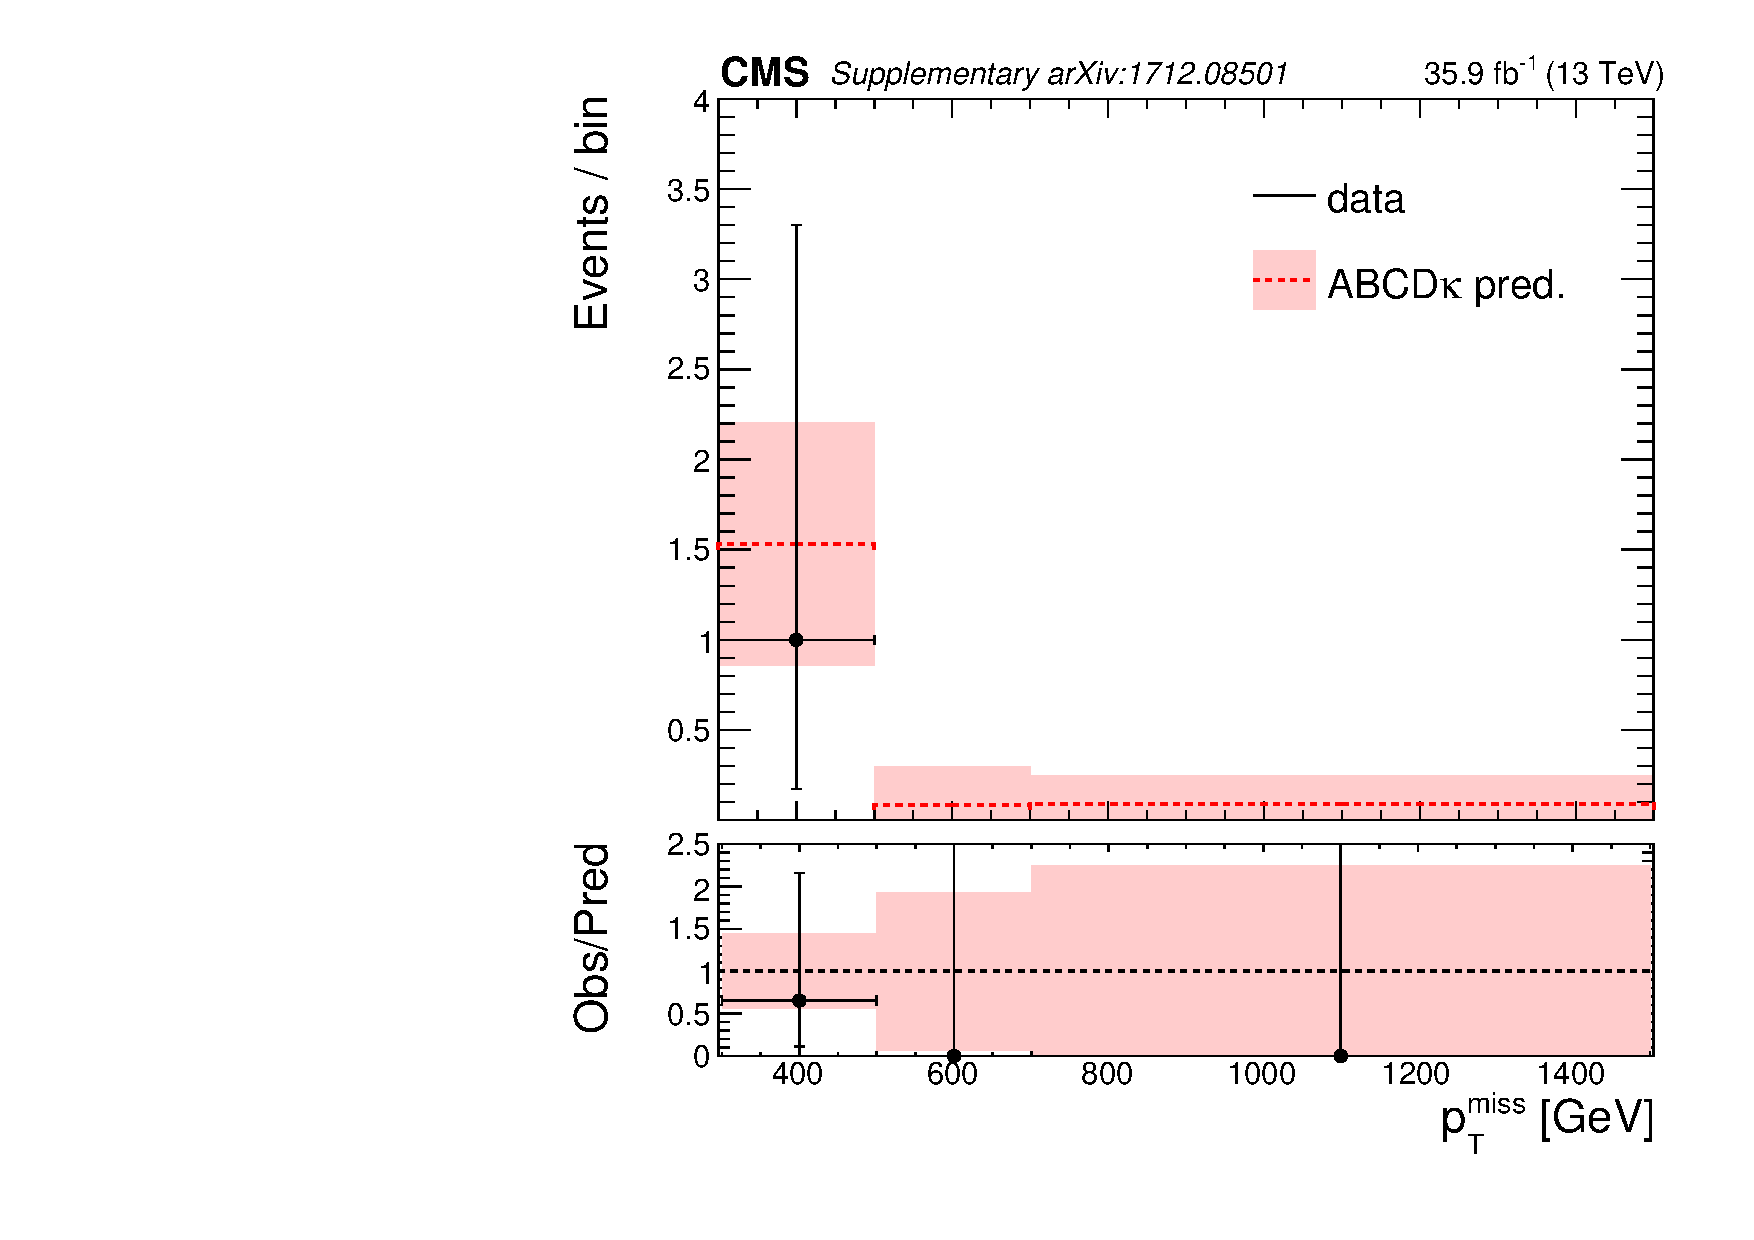
\includegraphics[width=0.75\textwidth]{figs/CMS-SUS-17-006_Figure-aux_005.pdf}
\caption{Two Higgs tag (A2)}
\end{subfigure}

\caption{Observed yields in the single and double Higgs-tagged signal regions.}
\label{fig:signalyields}
\end{figure}

\begin{table}[htbp]
\centering
\caption{Observed yields in signal and control regions, along with the background predictions.}
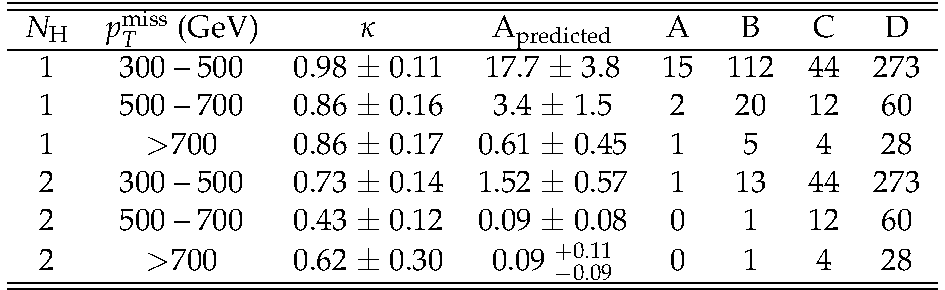
\includegraphics[width=0.75\textwidth]{figs/CMS-SUS-17-006_Table-aux_001.pdf}
\label{tab:yieldstable}
\end{table}

Interpreting our results in the context of the T5HH or T5ZH models, the absence of signal allows us to place limits on the masses of the Supersymmetric particles. Assuming a mass of 1 GeV for the neutralino $\chi_{1}^{0}$, and a small mass splitting of 50 GeV between the gluino and neutralino $\chi_{2}^{0}$, we are able to place lower limits at 95\% confidence level on the gluino mass at 2010 and 1825 GeV for the T5HH and T5ZH models, respectively. The exclusion curves are seen in Figure \ref{fig:brazil}. The weaker limit for the T5ZH model is due to the smaller branching fraction of the Z boson to b-quarks and our choice of signal mass window not being optimal for a Z boson.

\begin{figure}[htbp]
\centering
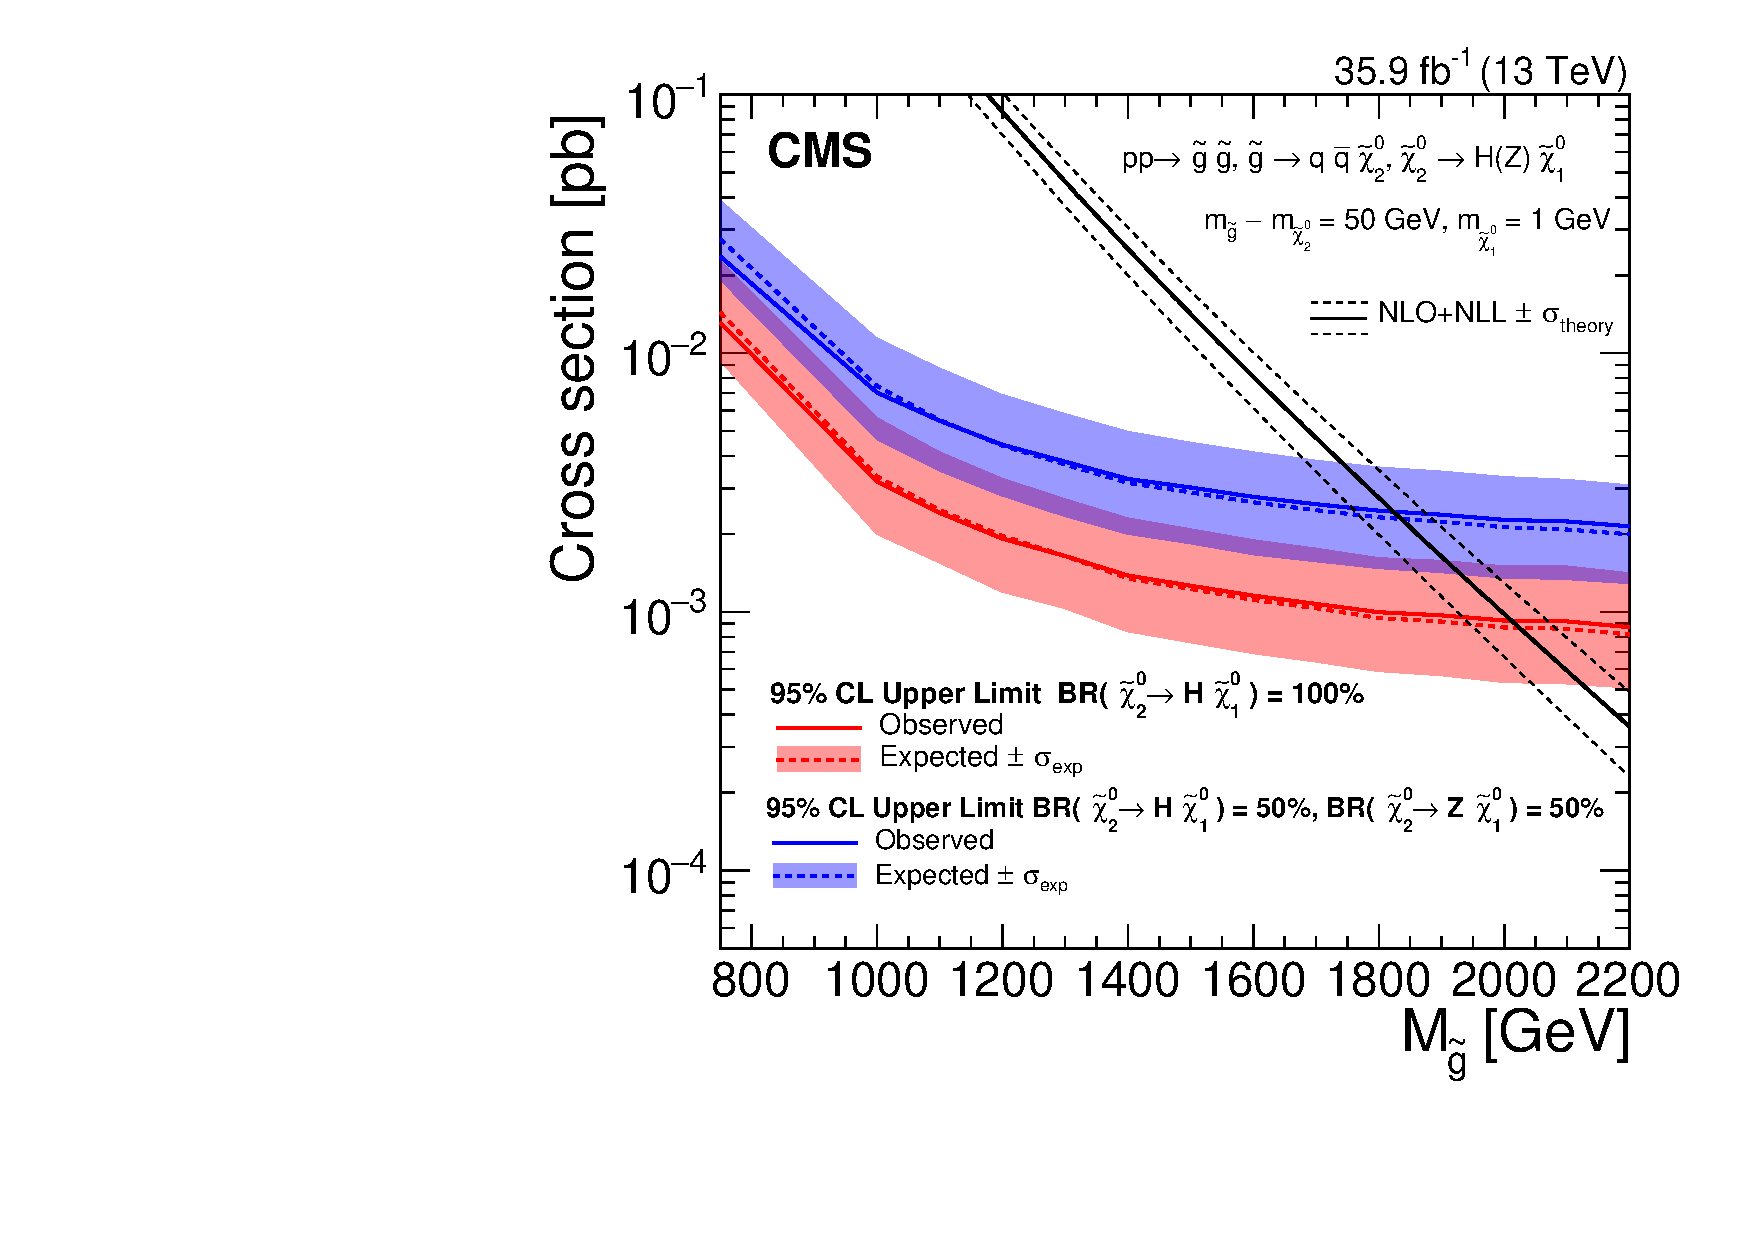
\includegraphics[width=0.75\textwidth]{figs/CMS-SUS-17-006_Figure_003.pdf}
\caption{Observed and expected limits on the gluino cross section when the data are interpreted in the T5HH and T5HZ models.}
\label{fig:brazil}
\end{figure}
